This section presents a summary of the results from previous chapters, lists
important results and discoveries, and suggests contributions made to computer
science by this project.

\section{Cache Results}

The test results in this project mostly agreed with LaMarca's results.  The
heapsort graphs had nearly exactly the same shape as LaMarca's, and the ratios
between the base and cache-conscious versions were nearly identical. The
multi-mergesort results were slightly different: instruction count was
identical, but while the cache results of the base and tiled mergesorts were
identical, multi-mergesort results were not the same. However, the basis for
those results - a sharp increase in cache misses followed by a flat-lined graph
- were in both cases.

The quicksort results were also very similar, though the multi-quicksort results
had a slightly different shape to LaMarca's. However, the instruction count
results for each quicksorts agreed with LaMarca's results, as did cache miss
results of the base and cache-conscious versions.

The two sets of radixsort results were slightly similar. The rise and plateau of
the curve to the right of the graphs was the same in both cases, though the left
hand side of the graphs did not agree.

Another interesting observation can be made: the results of the simulations on
the Pentium 4 were not always influenced by the cache misses. Though heapsort
and radixsort began to perform poorly once the data set no longer fit in the
cache, neither quicksort nor mergesort were affected. The reason why radixsort
was affected is obvious - there is no temporal reuse; in heapsort, the full
cache line is not being used, and spatial locality suffers as a result. It is
interesting that the other two sorts were unaffected, even though their cache
miss graphs indicate a significant increase in misses.

Finally, it was shown that in some cases a direct-mapped cache performed better
than a fully-associative one. The reasons for this were not clear.

\section{Branch Prediction Results}

Insertion sort has only one branch misprediction per key. This shows that it is
possible to predict comparative branches correctly, though the instruction cost
of such an algorithm may be high. This is also shown in multi-quicksort: though
the instruction count and memory reference count are both doubled, it is still
faster to use a sequential search than a binary search across small lists.

Selection sort has a similar number of instructions and cache misses as
bubblesort and a larger instruction and cache miss count than shakersort, yet it
still considerably outperforms both of these. This shows the high cost of branch
mispredictions on an algorithm.

Radixsort has almost no branch mispredictions at all. The only mispredictions
are due to its flow control, but it escapes comparative mispredictions, and this
factor allows it to perform as fast as, and in some cases faster than quicksort,
despite its high number of cache misses.

The heapsort results show the disadvantage of using unsorted lists. Even though
there are less branches in the 4-heap version, the number of branch
mispredictions are higher than in a standard 2-heap.

It is also shown that bimodal branch predictors generally out-perform two-level
adaptive predictors when resolving comparative misses. This is shown by the
results of insertion sort, bubblesort, shakersort, heapsort and quicksort. In
the cases where the two-level adaptive predictor does perform as well, the table
required is much larger than that required by the bimodal predictors to get the
same results.

\section{Best Sort}
The results also helped answer the question of which is the best sort. However,
it is important to remember that sorts have different purposes and properties,
so this shall be considered. A comparative chart of the fastest sorts is shown
in Figure \ref{All cycles}. This shows the cycles per key of each of the major
sorts and their derivatives, measured using Pentium 4 performance counters.
Neither the elementary sorts nor heapsorts are on the chart, as their results
are significantly worse than the other results, which makes it difficult to
accurately see those results.

\afterpage{
\thispagestyle{empty}
\clearpage
\enlargethispage{14em}
\vspace*{-10em}
\setcounter{figure}{8}
\begin{figure}[H]
\begin{changemargin}
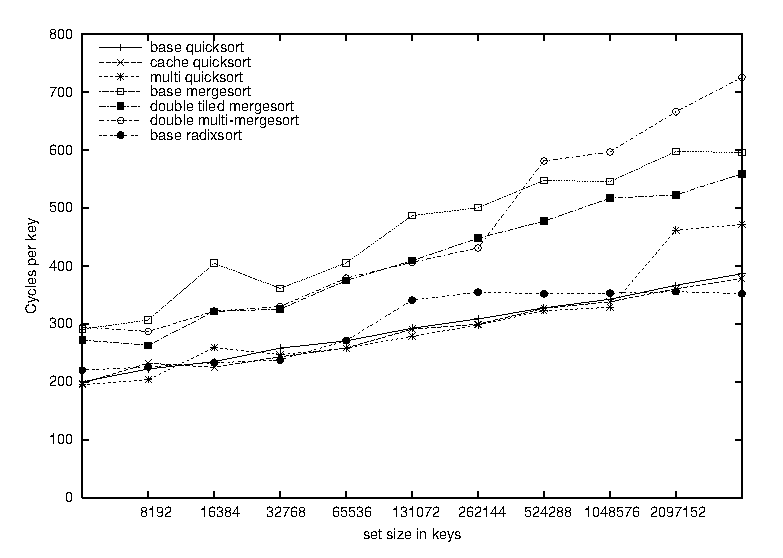
\includegraphics[angle=90,scale=1.8]{plots/all_cycles}
\vspace*{8em}
\end{changemargin}
\caption{\label{All cycles}Cycles per key of several major sorts and their variations - this was
measured on a Pentium 4 using hardware performance counters.}
\end{figure}
\newpage
}

The best stable sort is radixsort. The best comparison-based stable sort is
double tiled mergesort. The best in-place sort is quicksort. The best in-place
stable sort is, sadly, insertion sort. The best elementary sort is also
insertion sort; as such it should be only used for very small data sets.  The
best sort for very large data sets is radixsort. The best overall sort was
quicksort, though radixsort is very close, and the radixsort considered here was
not optimised. It is expected that an optimised radixsort would beat quicksort
for smaller sets.

\section{Contributions}

This section lists the contributions of this project. Each of these is novel  
and was discovered or developed during the course of this project.

The primary contribution of this project is that it repeats the work of LaMarca
on cache-conscious sorting, and validates many of his claims, while questioning
others. The next most important contribution is having performed a branch
prediction analysis of major sorts - which to my knowledge has not been done
before - and developing a framework by which these results can be repeated and
expanded upon.

Several discoveries were made and analysed: insertion sort has one misprediction
per key; selection sort has $log_2(N/2)$ branch mispredictions per key - an
explanation of this was also provided; tiling mergesort can be done in two
steps, reducing the cache miss count; it is possible to avoid using a
sentinel and still remove the bounds check from a standard 2-heap, simply by
reordering the steps involved; sequential searches are far cheaper than binary
searches across small lists, due to a low branch misprediction rate.

In addition, several ideas were conceived although not implemented, which relate
to sorting algorithms: it should be possible to reduce the conflict misses of
tiled mergesort without padding, by slightly reducing the size of the array
segments sorted in the first sorting phase; it may be possible to reduce the
cost of an insertion sort or selection sort by considering more than one key at
a time; it may be possible to reduce the number of partitions - and hence the
increase in instruction count - of multi-quicksort by choosing from a larger
selection of pivots. Finally, it should be possible to reduce by half the number
of cache misses in radixsort, by counting earlier and by copying back and forth
between two arrays.
